
\documentclass[11pt,letterpaper]{article}\usepackage[]{graphicx}\usepackage[]{color}
%% maxwidth is the original width if it is less than linewidth
%% otherwise use linewidth (to make sure the graphics do not exceed the margin)
\makeatletter
\def\maxwidth{ %
  \ifdim\Gin@nat@width>\linewidth
    \linewidth
  \else
    \Gin@nat@width
  \fi
}
\makeatother

\definecolor{fgcolor}{rgb}{0.345, 0.345, 0.345}
\newcommand{\hlnum}[1]{\textcolor[rgb]{0.686,0.059,0.569}{#1}}%
\newcommand{\hlstr}[1]{\textcolor[rgb]{0.192,0.494,0.8}{#1}}%
\newcommand{\hlcom}[1]{\textcolor[rgb]{0.678,0.584,0.686}{\textit{#1}}}%
\newcommand{\hlopt}[1]{\textcolor[rgb]{0,0,0}{#1}}%
\newcommand{\hlstd}[1]{\textcolor[rgb]{0.345,0.345,0.345}{#1}}%
\newcommand{\hlkwa}[1]{\textcolor[rgb]{0.161,0.373,0.58}{\textbf{#1}}}%
\newcommand{\hlkwb}[1]{\textcolor[rgb]{0.69,0.353,0.396}{#1}}%
\newcommand{\hlkwc}[1]{\textcolor[rgb]{0.333,0.667,0.333}{#1}}%
\newcommand{\hlkwd}[1]{\textcolor[rgb]{0.737,0.353,0.396}{\textbf{#1}}}%

\usepackage{framed}
\makeatletter
\newenvironment{kframe}{%
 \def\at@end@of@kframe{}%
 \ifinner\ifhmode%
  \def\at@end@of@kframe{\end{minipage}}%
  \begin{minipage}{\columnwidth}%
 \fi\fi%
 \def\FrameCommand##1{\hskip\@totalleftmargin \hskip-\fboxsep
 \colorbox{shadecolor}{##1}\hskip-\fboxsep
     % There is no \\@totalrightmargin, so:
     \hskip-\linewidth \hskip-\@totalleftmargin \hskip\columnwidth}%
 \MakeFramed {\advance\hsize-\width
   \@totalleftmargin\z@ \linewidth\hsize
   \@setminipage}}%
 {\par\unskip\endMakeFramed%
 \at@end@of@kframe}
\makeatother

\definecolor{shadecolor}{rgb}{.97, .97, .97}
\definecolor{messagecolor}{rgb}{0, 0, 0}
\definecolor{warningcolor}{rgb}{1, 0, 1}
\definecolor{errorcolor}{rgb}{1, 0, 0}
\newenvironment{knitrout}{}{} % an empty environment to be redefined in TeX

\usepackage{alltt}
\usepackage[utf8]{inputenc}
\usepackage{authblk}
\usepackage{multicol}
\usepackage{graphicx}
\usepackage[unicode=true]{hyperref}
\hypersetup{breaklinks=true,
            bookmarks=true,
            colorlinks=true,
            citecolor=blue,
            urlcolor=blue,
            linkcolor=magenta,
            pdfborder={0 0 0}}
\urlstyle{same}
\setlength{\columnsep}{1cm}
\usepackage[left=1.5cm,right=1.5cm,top=1.5cm,bottom=1.5cm]{geometry}
\title{\textbf{Risk Groups Systems for Penile Cancer Management: A Study of 203 Patients with Invasive Squamous Cell Carcinoma}}
\author{Alcides Chaux, M.D.\textsuperscript{1,2}}
\date{}
\IfFileExists{upquote.sty}{\usepackage{upquote}}{}
\begin{document}

\maketitle

\begin{abstract}
The aim of the current study was to evaluate the accuracy of previously published risk groups systems for predicting inguinal nodal metastases in patients with penile carcinoma. For this, 203 cases of invasive penile squamous cell carcinomas were stratified using the following systems: Solsona \emph{et al} (J Urol 2001;165:1509), Hungerhuber \emph{et al} (Urology 2006;68:621), and the proposed by the European Association of Urology (Eur Urol 2004;46:1). Each of these system allocated patients with penile cancer in low, intermediate, and high risk categories for inguinal nodal metastasis. Metastatic rates and cancer-specific survival rates of patients in the dataset were compared with previously reported results. Receiver-operator characteristic (ROC) curves were generated to compare accuracy in predicting final nodal status and cancer-related death. Most of cases were pT2/pT3 high-grade tumors with a small percentage of low grade pT1 carcinomas. The metastatic rates for the Solsona \emph{et al}, EUA, and Hungerhuber \emph{et al} systems in the high risk category were 15/73 (21\%), 16/103 (16\%), and 10/35 (29\%) patients with clinically negative inguinal lymph nodes and 52/75 (69\%), 55/93 (59\%), and 34/47 (72\%) patients with palpable inguinal lymph nodes, respectively. Performance by ROC curves analysis showed a low accuracy for all stratification systems although the Solsona \emph{et al} and the Hungerhuber \emph{et al} systems performed better than the EAU system. Patients in intermediate risk categories and with clinically palpable inguinal lymph nodes were more likely to have nodal metastasis than patients with clinically negative lymph nodes in the same category. In conclusion, these stratification systems may be useful for patients with low-grade superficial tumors and less accurate for evaluating patients with high-grade locally-advanced penile carcinomas. These data may be useful for therapeutic planning of patients with penile squamous cell carcinomas.
\\\\
\textbf{Keywords:} penile squamous cell carcinoma; prognostic factors; risk group stratification systems; prognosis; inguinal metastasis.
\end{abstract}

\let\thefootnote\relax\footnote{
\\ \textbf{Author Affiliation:} \textsuperscript{1}Department of Scientific Research, Norte University, Paraguay; \textsuperscript{2}Centro para el Desarrollo de la Investigación Científica, Asunción, Paraguay.
}
\let\thefootnote\relax\footnote{
\\ \textbf{Corresponding Author:} Alcides Chaux, M.D. Department of Scientific Research, Norte University, Gral. Santos e/ 25 de Mayo, Asunción, Paraguay. Office: +595 (021) 203-108, ext. 142. Email: \href{mailto:alcideschaux@uninorte.edu.py}{alcideschaux@uninorte.edu.py}
}

\begin{multicols}{2}
\section*{Introduction}
Regional nodal metastasis is the most important adverse prognostic factor defining outcome in penile squamous cell carcinoma (SCC) \cite{Novara2007,Chaux2009}. However, about one-half of patients who receive an inguinal lymphadenectomy as part of penile cancer treatment develop significant complications \cite{Spiess2009}. On this regard, several non-invasive and minimally invasive diagnostic approaches have been attempted to better define which group of patients will benefit the most from a groin dissection \cite{Hughes2009}. The identification of the sentinel node using radioactive tracers and gamma-probes, a procedure named ``dynamic sentinel lymph node biopsy'' (DSLNB), has given promising results in some specialized centers \cite{Leijte2007}. With this technique, and in selected cases, the status of the sentinel node is used to decide whether or not a groin dissection should be performed. However, the high costs, infrastructure, and technical expertise required for the procedure may preclude its worldwide implementation. In addition, to overcome the complications associated with a groin dissection, novel techniques such as video endoscopic inguinal lymphadenectomy have been developed \cite{Sotelo2009}. Nonetheless, there is neither general consensus nor uniform results regarding formal indications or most suitable surgical techniques. Thus, the ideal management of regional lymph nodes in penile cancer remains controversial.

Aimed at predicting the likelihood of nodal metastasis several pathologically-based risk groups stratification systems have been constructed and evaluated \cite{Solsona2004,Solsona2001,Hungerhuber2006,Hegarty2006}. These predictive tools seek to offer clinically-significant guidance in the decision of whether to perform or not an inguinal lymphadenectomy. They combine the prognostic value of histological grade and depth of tumor infiltration, both considered among the most useful parameters to predict nodal metastasis \cite{Chaux2009,Velazquez2008,Slaton2001,Dai2006,Chaux2009b}. According to these risk groups systems, patients in a high risk category should receive a groin dissection as part of primary treatment while with patients in a low risk category a follow-up and surveillance program would suffice \cite{Solsona2004,Solsona2001,Hungerhuber2006}. The aim of this study was to comparatively assess the performance of the proposed systems in predicting inguinal metastasis and defining discrete survival groups. For this purpose we used a cohort of patients from a geographical region of high incidence in penile cancer.

\section*{Material \& Method}
\subsection*{Cohort of Patients}
Patients were selected from a previously published series of 333 patients with invasive penile squamous cell carcinoma \cite{Guimaraes2009}. This dataset is publicly available at \href{http://dx.doi.org/10.6084/m9.figshare.1290997}{http://dx.doi.org/10.6084/m9.figshare.1290997}. Only patients with total or partial penectomy were included. Cases with missing values in the variables \emph{histologic grade} and \emph{pT stage} were excluded. Patients who were lost at follow-up were also excluded. The final count of selected cases for data analysis was 203.

\subsection*{Tumor Depth and Histologic Grade}
Deepest anatomical extension of the tumor was microscopically confirmed and the following anatomical levels were established: lamina propria (LP), corpus spongiosum (CS) and corpus cavernosum (CC). Histological grades were assigned according to previously reported and validated criteria \cite{Velazquez2008,Chaux2009b}, as follows: grade 1, tumor entirely composed of neoplastic cells resembling normal squamous cells with minimal basal/parabasal nuclear atypia; grade 2, tumors not fitting criteria for grade 1 or grade 3; grade 3, tumors composed of any proportion of anaplastic cells showing nuclear pleomorphism, coarse chromatin, prominent nucleolus, irregular and thickened nuclear membrane, with abundant and/or atypical mitoses.

\subsection*{Clinical and Pathological Staging}
Clinical and pathological staging were carried out using the latest TNM classification system \cite{Hakenberg2015}. Clinical staging of inguinal lymph nodes included the following categories: cN0, no palpable inguinal nodes; cN1, palpable mobile unilateral inguinal lymph node; cN2, palpable mobile multiple or bilateral inguinal lymph nodes; cN3, unilateral or bilateral palpable fixed inguinal nodal mass or pelvic lymphadenopathy. Clinically positive inguinal nodes (cN+) included cN1, cN2, and cN3 stages.

For pathological staging the following categories were used: pT1, tumors invading up to subepithelial connective tissue (lamina propria); pT2, tumors invading either corpus cavernosum or spongiosum, with or without lymphovascular invasion; and, pT3, tumors invading penile distal urethra. Urethral invasion was considered positive when tumor was identified within the urethral mucosa, either as an intraepithelial spread or infiltrating lamina propria.

\subsection*{Follow-Up}
Patients were followed-up from 0.8 to 433.9 months (mean, 108.1 months; median, 86.8 months). Two endpoints were evaluated during follow-up:
\begin{enumerate}
        \item \textbf{Tumor relapse:} tumor relapse included the development of local relapse (i.e., tumor on stump), regional relapse (i.e., metastases in regional lymph nodes), or systemic relapse (i.e., metastases in systemic lymph nodes, visceral metastases) during follow-up.
        \item \textbf{Outcome:} the possible categories of outcome included alive without disease, alive with disease, died of other causes, and died of cancer.
\end{enumerate}

\begin{table*}
\centering
        \caption{Distribution of tumors by pT stage and histologic grade in previously reported and current series}
        \label{Distribution_Table}
\begin{tabular}{lcccc}
\hline 
\ & Solsona \emph{et al} & Hungerhuber \emph{et al} & Hegarty \emph{et al} & Current series \\
\hline
\textbf{No. Cases} & 37 & 56 & 100 & 203 \\
\textbf{pT stage} & \ & \ & \ & \ \\
        \hspace{2ex}Tis/T1    & 18 (49\%)   & 30 (54\%)   & 28 (28\%)   & 8 (4\%) \\
        \hspace{2ex}T2        & 16 (43\%)   & 18 (32\%)   & 33 (33\%)   & 107 (53\%) \\
        \hspace{2ex}T3        & 3 (8\%)     & 8 (14\%)    & 39 (39\%)   & 88 (43\%) \\
\textbf{Histologic grade } & \ & \ & \ & \ \\
        \hspace{2ex}Grade 1   & 20 (54\%)   & 10 (18\%)   & 39 (44\%)   & 52 (26\%) \\
        \hspace{2ex}Grade 2   & 13 (35\%)   & 27 (48\%)   & 35 (40\%)   & 69 (34\%) \\
        \hspace{2ex}Grade 3   & 4 (11\%)    & 19 (34\%)   & 14 (16\%)   & 82 (40\%) \\
\hline 
\end{tabular}
\end{table*}

\subsection*{Final Lymph Nodes Status}
The final status of inguinal lymph nodes was established as follows: 
\begin{enumerate}
        \item \textbf{Positive status:} the final nodal status was considered positive if pathologically-proven nodal metastases were observed (in those cases with inguinal lymphadenectomy), if regional relapse appeared during follow-up, or if the outcome was unfavorable (i.e., alive with disease or death by cancer).
        \item \textbf{Negative status:} the final nodal status was considered negative if nodal metastases were not observed (in those cases with inguinal lymphadenectomy), if no tumor relapse (beyond local relapse) appeared during follow-up, or if the outcome was favorable (i.e., alive without disease or death by other causes).
\end{enumerate}

\subsection*{Risk Groups}
Risk groups were built using previously reported criteria and consisted of a combination of histological grade and tumor extension \cite{Solsona2004,Solsona2001,Hungerhuber2006}. Stratification was as it follows:

\textbf{Solsona \emph{et al} system \cite{Solsona2001}:} Tumors with grade 1 and pT1 stage were assigned to the low risk category, while tumors with grade 2 or 3 and pT2 or pT3 stage were considered part of the high risk category. The remaining cases (grades 2 or 3 with a pT1 stage or pT2/pT3 tumors with grade 1) were assigned to the intermediate category.

\textbf{European Association of Urology (EAU) system \cite{Solsona2004}, evaluated by Hegarty \emph{et al} \cite{Hegarty2006}:} pT1 with grade 1 tumors were assigned to the low risk category; grade 3 tumors (regardless of pT stage) or pT2/pT3 stage (regardless of histologic grade) were considered high risk tumors, while grade 2 and pT1 were in the intermediate category.

\textbf{Hungerhuber \emph{et al} system \cite{Hungerhuber2006}:} Tumors with grade 3 were considered high risk, regardless of the pT stage; pT1 stage tumors with grades 1 or 2 were assigned to the low risk category. The remaining cases (pT2 or pT3 with grades 1 or 2 tumors) were considered part of the intermediate category.

\subsection*{Statistical analyses}
Bivariate analyses were carried out using Fisher's exact test. Survival curves were generated using the Kaplan-Meier method and compared with the log-rank (Mantel-Cox) test. Each stratification system was confronted with the others to evaluate its diagnostic accuracy using Receiver-Operator Characteristic (ROC) curves. The area under the ROC curve (AUC) and the 95\% confidence interval were reported. Criteria for classifying the accuracy of ROC curves were those defined by Collinson \cite{Collinson1998}, as follows: 0.50\textendash 0.70, low accuracy; 0.71\textendash 0.90, moderate accuracy; and \textgreater 0.90, high accuracy. The Mann-Whitney test was used to evaluate if ROC curves were significantly different from $AUC = 0.5$. In all cases a 2-tailed $P\textless 0.05$ was required for statistical significance. Data were analyzed and plots were generated using R version 3.1.1 ``Sock it to Me'' \cite{RCoreTeam}. ROC curves analysis was carried out using the \texttt{pROC} package \cite{Robin2011}. The dataset and R scripts used for data analysis, as well as additional results (including the full analysis of the dataset), are freely available at \href{https://github.com/alcideschaux/Penis-RiskGroups}{github.com/alcideschaux/Penis-RiskGroups}.

\begin{table*}
\centering
        \caption{Final nodal status according to risk group stratification systems}
        \label{FinalNodal}
\begin{tabular}{lcccc}
\hline 
Risk Group System & Previously Reported & cN0 & cN+ & All Patients \\
\ & \ & 108 & 95 & 203 \\
\hline
\textbf{Solsona \emph{et al} system} & \ & \ & \ & \ \\
        \hspace{2ex}High risk & 10/12 (83\%)
                & 15/73 (21\%)
                & 52/75 (69\%)
                & 67/148 (45\%) \\
        \hspace{2ex}Intermediate risk & 4/12 (33\%)
                & 1/32 (3\%)
                & 3/18 (17\%)
                & 4/50 (8\%) \\
        \hspace{2ex}Low risk & 0/13 (0\%)
                & 0/3 (0\%)
                & 0/2 (0\%)
                & 0/5 (0\%) \\
\textbf{EAU system} & \ & \ & \ & \ \\
        \hspace{2ex}High risk & 23/74 (31\%)
                & 16/103 (16\%)
                & 55/93 (59\%)
                & 71/196 (36\%) \\
        \hspace{2ex}Intermediate risk & 0/9 (0\%)
                & 0/2 (0\%)
                & 0/0 % No cN+ patients in the intermediate category
                & 0/2 (0\%) \\
        \hspace{2ex}Low risk & 0/17 (0\%)
                & 0/3 (0\%)
                & 0/2 (0\%)
                & 0/5 (0\%) \\
\textbf{Hungerhuber \emph{et al} system} & \ & \ & \ & \ \\
        \hspace{2ex}High risk & 3/4 (75\%)
                & 10/35 (29\%)
                & 34/47 (72\%)
                & 44/82 (54\%) \\
        \hspace{2ex}Intermediate risk & 2/7 (29\%)
                & 6/68 (9\%)
                & 21/46 (46\%)
                & 27/114 (24\%) \\
        \hspace{2ex}Low risk & 1/13 (8\%)
                & 0/5 (0\%)
                & 0/2 (0\%)
                & 0/7 (0\%) \\
\hline 
\end{tabular}
\end{table*}


\section*{Results}
Distribution of tumors by T stage and histological grade in previously reported and current cohort is shown in Table \ref{Distribution_Table}. Most cases in the Solsona \emph{et al} and the Hungerhuber \emph{et al} series were located in the pT1 stage while a minority corresponds to pT3 tumors. The opposite was observed in our cohort, with a small percentage of cases in the pT1 category and most tumors in the pT2/pT3 stage. The distribution of pathological stages in the EAU system was similar among categories. Regarding histological grade, high-grade (grade 3) tumors were more prevalent in our series than in all the others while low-grade tumors (grade 1 and 2) predominated in the previously reported series.

\subsection*{Final Lymph Nodes Status}
Distribution according to cN stage was as it follows: 108 patients (53\%) were cN0, 31 (15\%) were cN1, 59 (29\%) were cN2, and 5 (2\%) were cN3. The final nodal status was positive in 71 (35\%) of all cases. Regarding histologic grade, the final nodal status was positive in 4/52 (8\%) of grade 1 tumors, 23/69 (33\%) of grade 2 tumors, and 44/82 (54\%) of grade 3 tumors. The association between histologic grade and final nodal status was statistically significant (Fisher's exact $P=7.6e-08$).

Regarding pT stage, the final nodal status was positive in 0/8 (0\%) of pT1 tumors, 31/107 (29\%) of pT2 tumors, and 40/88 (45\%) of pT 3 tumors. The association between pT stage and final nodal status was statistically significant (Fisher's exact $P=0.0044$). Table \ref{FinalNodal} summarizes the final nodal status by risk group systems and cN status.

\textbf{Solsona \emph{et al} system:} 148 (73\%) of patients were located in the high risk category, 50 (25\%) in the intermediate category, and 5 (2\%) in the low risk category. In the original series the distribution by risk groups was 32.5\%, 32.5\%, and 35\%, respectively \cite{Solsona2001}. Overall, the final nodal status was positive in 67/148 (45\%) patients in the high risk category, 4/50 (8\%) patients in the intermediate risk category, and 0/5 (0\%) patients in the low risk category. In the high risk and intermediate risk categories metastatic rates were higher in cN+ patients when compared with cN0 patients. No metastasis were found in the low risk categories, in both cN0 and cN+ patients. Compared to the previously reported rates ours were lower in the high and intermediate risk categories. The association between final nodal status and risk groups was statistically significant (Fisher's exact $P=2.4e-07$) when both cN0 and cN+ patients were taken into account. This association remained significant for cN+ patients (Fisher's exact $P=3.2e-05$) but not for cN0 patients (Fisher's exact $P=0.055$).

\textbf{EAU system:} 196 (97\%) of patients were located in the high risk category, 2 (1\%) in the intermediate category, and 5 (2\%) in the low risk category. The distribution of patients in the series of Hegarty \emph{et al} was 74\%, 9\%, and 17\%, respectively \cite{Hegarty2006}. Overall, the final nodal status was positive in 71/196 (36\%) patients in the high risk category, 0/2 (0\%) patients in the intermediate risk category, and 0/5 (0\%) patients in the low risk category. The metastatic rate in the high risk category was higher in cN+ patients when compared with cN0 patients. All the patients in the intermediate category were cN0 and none presented nodal metastasis. No metastasis were found in the low risk categories, in both cN0 and cN+ patients. Our rates were similar to those reported in the series of Hegarty \emph{et al}. The association between final nodal status and risk groups was not statistically significant for both cN0 and cN+ patients (Fisher's exact $P=0.21$), cN0 patients alone (Fisher's exact $P=1$), or cN+ patients alone (Fisher's exact $P=0.17$).

\textbf{Hungerhuber \emph{et al} system:} 82 (40\%) of patients were located in the high risk category, 114 (56\%) in the intermediate category, and 7 (3\%) in the low risk category. In the original series the distribution by risk groups was 17\%, 29\%, and 54\%, respectively \cite{Hungerhuber2006}. Overall, the final nodal status was positive in 44/82 (54\%) patients in the high risk category, 27/114 (24\%) patients in the intermediate risk category, and 0/7 (0\%) patients in the low risk category. In the high risk and intermediate risk categories metastatic rates were higher in cN+ patients when compared with cN0 patients. No metastasis were found in the low risk categories, in both cN0 and cN+ patients. Compared to the previously reported rates ours were lower in all the categories, except for cN+ in the intermediate category. The association between final nodal status and risk groups was statistically significant (Fisher's exact $P=7e-06$) when both cN0 and cN+ patients were taken into account. This association remained significant for cN+ patients (Fisher's exact $P=0.0047$) and for cN0 patients (Fisher's exact $P=0.028$).

\subsection*{Survival Analysis}
Figures \ref{fig:Survival_FN} and \ref{fig:Survival_DOD} show the survival curves for final nodal status and cancer-related death considering histologic grade, pT stage, cN stage, and the evaluated risk group systems. For final nodal status survival curves were significantly different for histologic grade, pT stage, cN positivity, and the Solsona \emph{et al} and Hungerhuber \emph{et al} systems. Among the risk group systems the Hungerhuber \emph{et al} system offered a better separation between survival curves (see Figure \ref{fig:Survival_FN}). A similar pattern was observed for cancer-related death considering clinicopathologic features and risk group systems, although P values were slightly larger (see Figure \ref{fig:Survival_DOD}).

\begin{figure*}
\centering
\begin{knitrout}
\definecolor{shadecolor}{rgb}{0.969, 0.969, 0.969}\color{fgcolor}
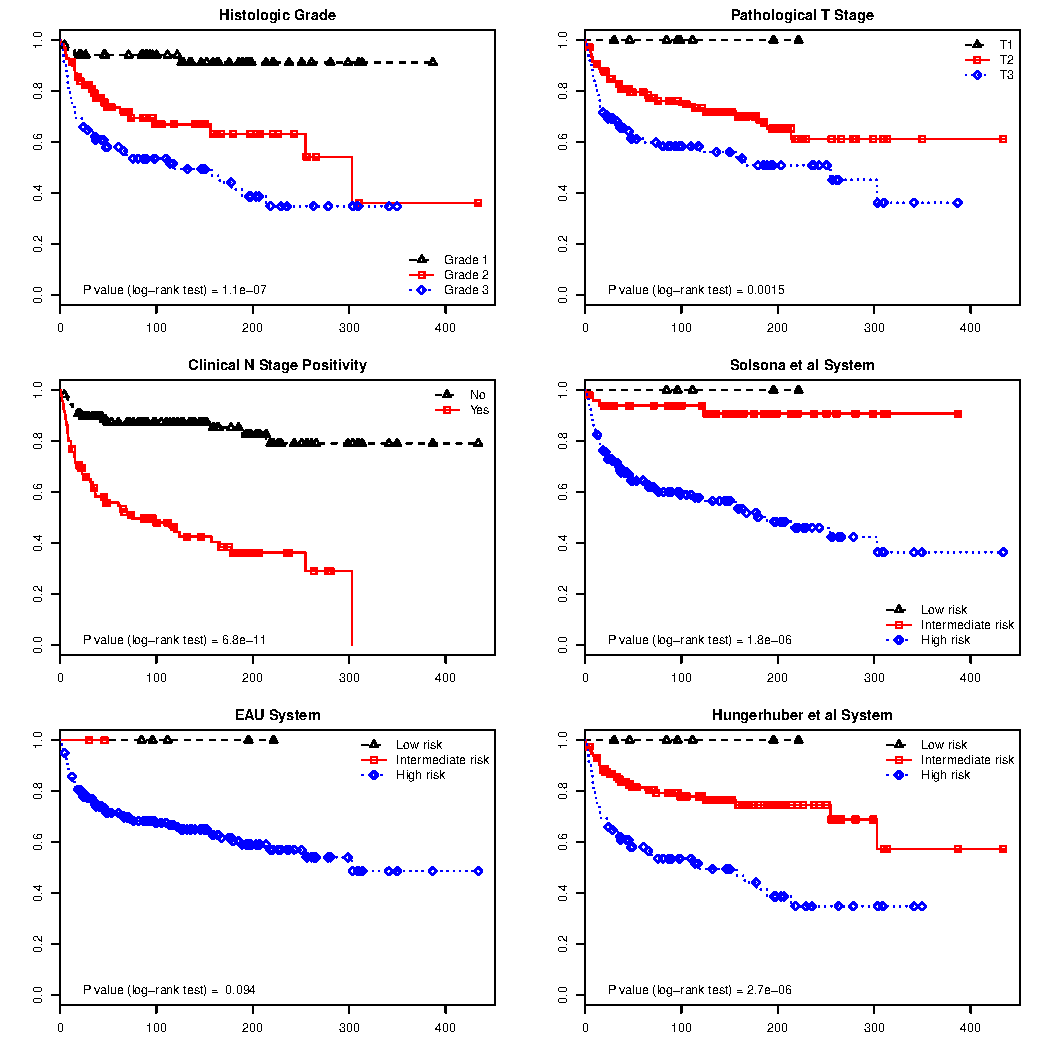
\includegraphics[width=\maxwidth]{figure/Survival_FN-1} 

\end{knitrout}
        \caption{Survival curves for final nodal status according to clinicopathologic features and risk group systems. Survival curves were significantly different for all variables except for the EAU system. Follow-up in months is depicted in the x-axes, while the y-axes depict survival functions.}
        \label{fig:Survival_FN}
\end{figure*}

\begin{figure*}
\centering
\begin{knitrout}
\definecolor{shadecolor}{rgb}{0.969, 0.969, 0.969}\color{fgcolor}
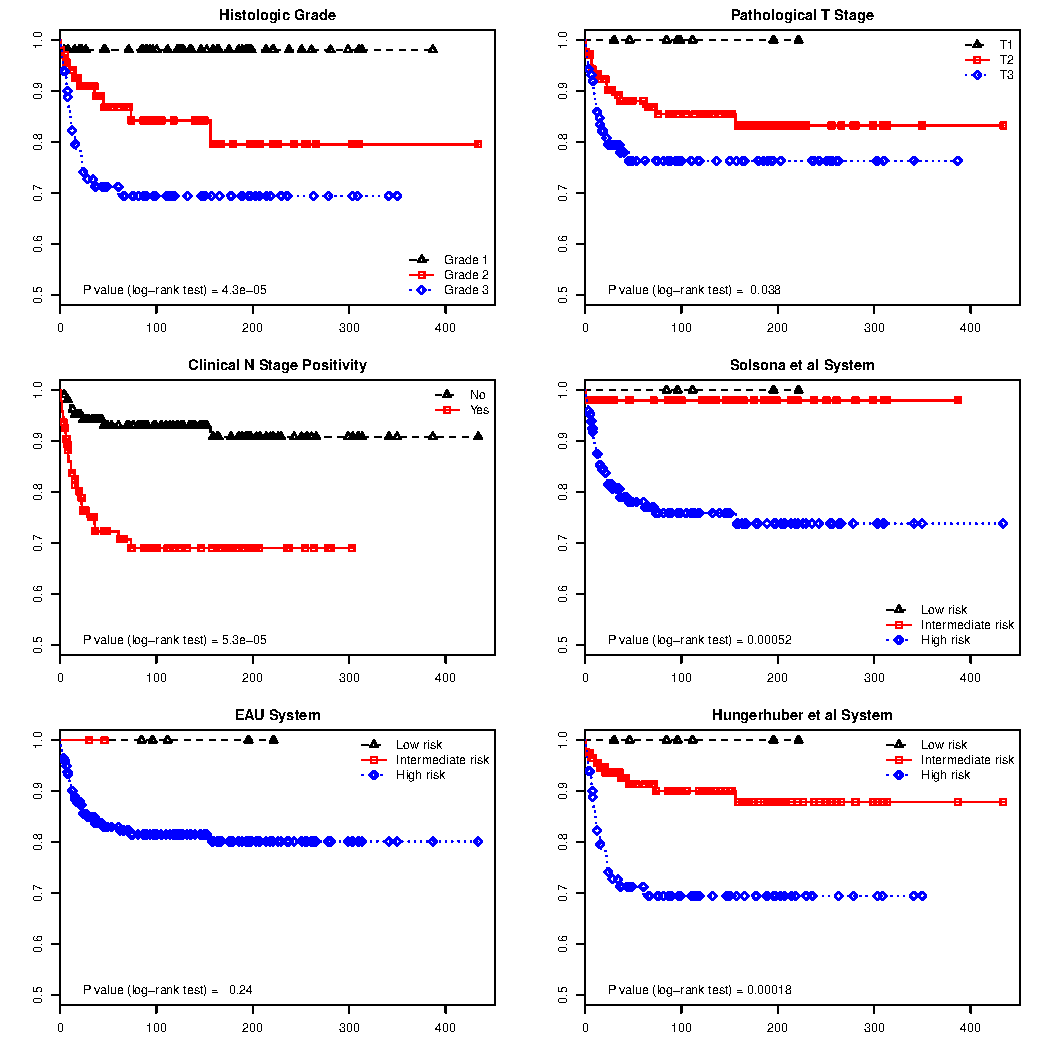
\includegraphics[width=\maxwidth]{figure/Survival_DOD-1} 

\end{knitrout}
        \caption{Survival curves for final nodal status according to clinicopathologic features and risk group systems. Survival curves were significantly different for all variables except for the EAU system. Follow-up in months is depicted in the x-axes, while the y-axes depict survival functions.}
        \label{fig:Survival_DOD}
\end{figure*}

\subsection*{ROC Curves Analysis}
Performance by ROC curves analysis (Table \ref{tab:ROC} and Figure \ref{fig:ROC}) showed a low accuracy for predicting final nodal status and cancer-related death in all systems, although the Solsona \emph{et al} and the Hungerhuber \emph{et al} systems performed better than the EAU system. AUC in the formers was also significantly different from 0.5 while in the latter the AUC did not significantly differ from 0.5 (see Table \ref{tab:ROC}).

\begin{table*}[t]
\centering
        \caption{Areas Under the ROC Curve for Final Nodal Status and Cancer-Related Death}
        \label{tab:ROC}
\begin{tabular}{lccc}
\hline
Risk Group System & Area Under the ROC Curve & 95\% CI & Mann-Whitney's P value \\
\hline
\textbf{Outcome: Final Nodal Status} & ~ & ~ & ~ \\
        \hspace{2ex}Solsona et al system 
                & 0.67
                & 0.62, 0.72
                & 4.6e-07 \\
        \hspace{2ex}EAU system
                & 0.53
                & 0.51, 0.55
                & 0.049 \\
        \hspace{2ex}Hungerhuber et al
                & 0.68
                & 0.61, 0.74
                & 2.1e-06 \\
\textbf{Outcome: Cancer-related death} & ~ & ~ & ~ \\
        \hspace{2ex}Solsona et al system
                & 0.65
                & 0.6, 0.69
                & 0.00054 \\
        \hspace{2ex}EAU system
                & 0.52
                & 0.51, 0.54
                & 0.23 \\
        \hspace{2ex}Hungerhuber et al system
                & 0.67
                & 0.59, 0.76
                & 0.00032 \\
\hline
\end{tabular}
\end{table*}

\section*{Discussion}
In this study we evaluated the performance of 3 risk groups systems built with the aim of predicting lymph node metastases and offering guidance in the clinical management of patients with penile cancer. Using a previously published dataset we found that the evaluated systems had a low accuracy, in spite of being significantly associated with the considered outcomes (i.e., final nodal status and cancer-related death). We also found different metastatic rates depending on the cN stage of the patients, suggesting that the clinical status of the inguinal lymph nodes should also be taken into account for adecuate management.

Groin dissection has proved to be an efficient method for controlling systemic dissemination of penile SCC, especially if done early in the course of the disease \cite{Hungerhuber2006,Kroon2005}. Nevertheless, criteria for deciding which patients should receive this procedure are not well established. As a first empirical approach risk groups could be built using clinicopathological features that have proven to be strongly associated with the presence of nodal metastases. However, recognizing these variables only solves part of the problem. Indeed, almost every pathological feature has been proposed as having more or less impact in the metastatic rate of penile SCC \cite{Novara2007,Chaux2012}. Nonetheless, criteria for diagnosing and categorizing each one of them are variable and groups of patients in which they are evaluated are not always homogeneous, precluding proper statistical meta-analyses. This, added to inherent biological, etiological, and perhaps geographical differences among different subtypes of penile SCC could explain the poor external validation. In addition, some features are not entirely independent from others or could even act as confounding variables. For instance, high grade tumors, such as basaloid, sarcomatoid and grade 3 usual-type SCC, tend to infiltrate deeper anatomical levels and are associated with a high mortality rate \cite{Guimaraes2009,Chaux2009a,Chaux2012}. However, this is not always the case since some low-grade deeply infiltrating tumors such as carcinoma cuniculatum and carcinomas with verrucous features are associated with a very low or even null rate of nodal involvement \cite{Guimaraes2009,Chaux2012,Barreto2007}. Histological grade seems to be more important than depth of invasion in these paradoxical tumors, a topic that merits further evaluation.

All evaluated systems use histological grade and tumor anatomical extension to define risk categories. Some of them give more weight to histological grade \cite{Hungerhuber2006}, some to anatomical extension \cite{Solsona2004}, and others combine both factors giving equal importance to each \cite{Solsona2001}. The selection of histological grade as a prognostic factor seems to be more than justified, given the strong association observed among increasing grades and higher metastatic and mortality rates, as found here and in other studies \cite{Slaton2001,Chaux2009b}. Nonetheless, a substantial interobserver variability has been reported when assigning histological grades to a tumor \cite{Naumann2009}. In the grading system used in the present study \cite{Chaux2009b} morphological criteria were strictly defined and emphasis was given to both ends of the differentiation spectrum, aiming to minimize variation among observers. Although we consider this approach would reduce subjectivity the external validation of the aforementioned grading system regarding interobserver and intraobserver agreement is still pending.

On the other hand, the current TNM system may not be adequate in some categories and could explain in part the low accuracy of the evaluated systems in terms of ROC curves analysis. Indeed, this system, which lumps invasion of corpus spongiosum and corpus cavernosum as a single pT2 category and considers urethral invasion as pT3, has received strong criticism \cite{Leijte2008,Leijte2009}. In a previous study we found that tumor invasion of corpus cavernosum is associated with a significantly higher metastatic rate when compared with tumors limited to corpus spongiosum \cite{Chaux2009}. Moreover, invasion of distal urethra is not necessarily indicative of aggressive behavior or worst prognosis and there is no rationale for considering urethral infiltration as an ominous sign \emph{per se}. On this regard, Leijte \emph{et al} have previously demonstrated the poor accuracy of the TNM system \cite{Leijte2009}. These authors propose a modification of the system in which invasion of corpus spongiosum is regarded as T2, invasion of corpus cavernosum as T3 and urethral invasion is no longer considered as an adverse prognostic factor. The use of this modified TNM system yields a higher accuracy compared with the AJCC/UICC TNM standard system. Unfortunately the currently-in-use TNM system for penile cancer still considers invasion of erectile tissues (either corpus spongiosum or cavernosum) as pT2 and regards invasion of distal urethra as pT3 \cite{Hakenberg2015}.

\begin{figure*}
\centering
\begin{knitrout}
\definecolor{shadecolor}{rgb}{0.969, 0.969, 0.969}\color{fgcolor}
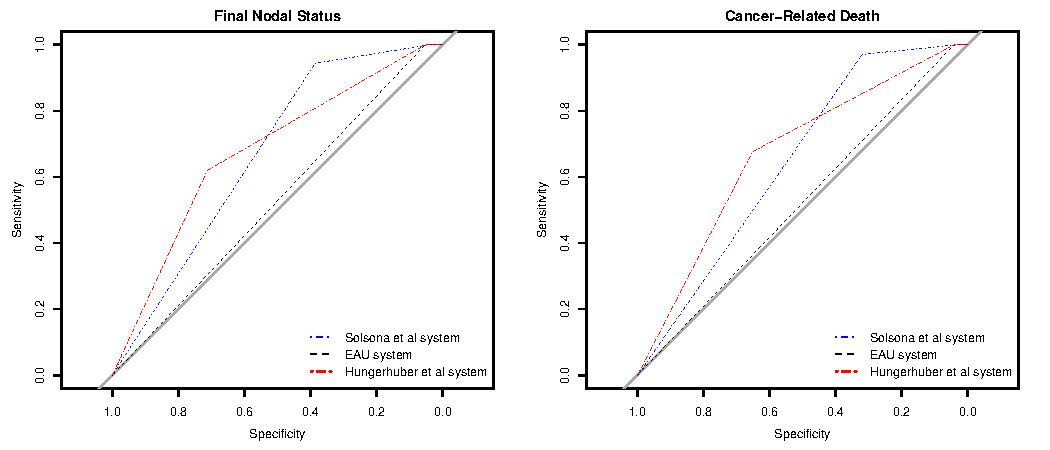
\includegraphics[width=\maxwidth]{figure/ROC-1} 

\end{knitrout}
        \caption{Receiver-operator characteristic (ROC) curves using final nodal status (left) and cancer-related death (right) as outcomes and the evaluated risk group systems as predictors.}
        \label{fig:ROC}
\end{figure*}

It is noteworthy the marked differences between the previously reported and currently found metastatic rates in cN0 patients using the Solsona \emph{et al} and Hungerhuber \emph{et al} systems. This finding could be explained by differences in pT stage. In both studies tumors with low pT stage predominate with about one-half of cases in Tis/T1 stage while tumors limited to lamina propria were infrequent in our series. This may indicate that in patients from geographical areas of low incidence penile tumors tend to be found in low pT stages whereas in areas of high incidence tumors are more locally advanced and consequently present a higher pT stage. Furthermore, the previously reported successfulness of the aforementioned systems could be biased by the fact that tumors were of low pT stage and the purportedly inherent failures of the TNM system were not apparent at this level. These shortcomings would manifest when tumors invading deep erectile tissues are considered, as in our current series. Perhaps these stratification systems are not appropriate to evaluate tumors with higher pT stage and other approaches are necessary. Another source of disparity can be found in histological grading. In none of the evaluated systems morphological criteria for grading were described in detail. Using strict and validated morphological criteria \cite{Chaux2009b} we found that most of our tumors were high grade. This is consistent with the higher pT stage of our tumors, since there is a strong association of high histological grade and depth of invasion \cite{Guimaraes2009}. 

The results of the current study are in agreement with those reported by Novarra \emph{et al} who evaluated the performance of the Solsona \emph{et al} and the EAU systems \cite{Novara2008}. They found that both systems had low predictive accuracy. Our analysis also shows that the Solsona \emph{et al} and the Hungerhuber \emph{et al} systems are similar in terms of accuracy while the EUA system showed the poorest performance in terms of predictive accuracy. ROC curves analysis indicates that maybe the latter system is not appropriate for predicting nodal involvement, at least in our cases. Again, these results can be best explained by the extreme importance given to the pT stage for defining EAU risk groups. Nonetheless, the use of risk groups systems should be encouraged since it allows the identification of patients at high-risk for nodal involvement.

In addition, the decision of whether to perform or not a groin dissection should also consider the clinical stage of the disease. In patients with impalpable lymph nodes the DSLNB procedure has proven useful but it has low accuracy when metastatic disease is clinically suspected \cite{Leijte2007,Kroon2005,Heyns2008,Hungerhuber2006a}. Our results also show that cN staging may provide useful information to complement risk groups systems, especially when patients in intermediate risk categories are considered. Indeed, and putting aside the EAU system, cN+ patients in intermediate categories were more likely to present nodal metastasis than cN0 patients in the same group. Perhaps when access to DSLNB or frozen sections are not available clinical staging of inguinal lymph nodes may provide a quick and inexpensive way to better allocate patients in intermediate categories. Although our data suggest that patients in low risk groups may be managed by surveillance alone and that no groin dissection is necessary, the small number of cases we have in these categories preclude more solid conclusions.

We have previously proposed an alternative to the evaluated risk group systems \cite{Chaux2009}. In this system 3 morphological variables (anatomical level of maximum tumor invasion, histological grade and presence of perineural invasion) are used to define three risk groups categories. Numerical values are assigned to each one of these variables and a score is obtained by adding them up. Using this system the inguinal metastatic rate is 0\% for the low risk category, 20\% for the intermediate risk category, and 64\% for the high risk category. In addition, scores obtained with this system are also useful to predict survival. Patients with scores 2 to 4 present a 5-year survival rate of 95\%. The survival rate of patients with scores 5 and 6 is 65\% while the score 7 is associated with a survival rate of only 45\%. Despite these results, this system needs yet to be externally validated and the findings confronted with new results obtained in large prospective series from geographical regions with low and high penile cancer incidence.

There are some limitations with the conclusions that may be drawn from our results. In the first place we used a retrospectively-collected series of cases and evaluation of the pT stage was done using only pathological reports and slides examination. This may have some impact in the proper staging of the disease. Second, the histological grading process was not uniform among previously reported series and we are not sure if our categories are comparable, and to what extent, with the ones assigned by the other authors. Both aforementioned shortcomings may have created discordances between the assignation of a particular case to one or another category depending on the criteria used either by the authors of the previous studies or by ourselves. Third, not all patients with penile cancer that were diagnosed, treated and followed-up could be included in the current study due to lack of pathological data regarding gross findings, adequate tissue sampling or proper follow-up in some of them. This may also have somehow biased our results. Notwithstanding these limitations, our study suggests that for deeply infiltrating penile carcinomas TNM-based stratification systems may not be appropriate and other clinicopathological variables should be taken into account.

In summary, 3 different risk group systems were evaluated in their accuracy for predicting final nodal status and their ability to define risk groups with different survival curves. Penile SCC from patients living in a geographical area of high penile cancer incidence seems to be of higher histological grade and pT stage when compared with patients in low-risk regions. The overall metastatic rates found in high risk categories were lower than those reported in the original series, either in cN0 or cN+ patients. We hypothesize that this may be related to the use of the TNM system for defining risk groups. Although in ROC curves analysis all of them rated as low accurate methods for predicting regional involvement they were useful in high risk cN+ patients. In addition, cN+ patients in intermediate categories are more likely to present nodal metastasis than those cN0 patients in the same category. Our findings suggest that these risk group systems may be appropriate for patients with low-grade superficial tumors and less useful for evaluating patients with high-grade locally-advanced penile carcinomas, although more studies are necessary to confirm these results.

\section*{Conflict of Interest}
The author declare no conflict of interest.

\section*{Financial Disclosure}
Dr. Alcides Chaux was partially supported by an award granted by the National Council of Science and Technology (CONACYT) dependent of the Presidency of the Republic of Paraguay, as a Level 2 Active Researcher of the National Incentive Program for Researchers (PRONII).

\bibliographystyle{unsrt}
\bibliography{References}

\end{multicols}
\end{document}
